\pdfminorversion=4
% Created 2017-05-31 mer. 10:21
\documentclass[smaller]{beamer}
\usepackage[utf8]{inputenc}
\usepackage[T1]{fontenc}
\usepackage{fixltx2e}
\usepackage{graphicx}
\usepackage{longtable}
\usepackage{float}
\usepackage{wrapfig}
\usepackage{rotating}
\usepackage[normalem]{ulem}
\usepackage{amsmath}
\usepackage{textcomp}
\usepackage{marvosym}
\usepackage{wasysym}
\usepackage{amssymb}
\usepackage{hyperref}
\tolerance=1000
\usepackage[T1]{fontenc}
\usepackage[english, frenchb]{babel}
\useoutertheme{infolines}
\mode<beamer>{\usetheme{Pittsburgh}}
\setbeamertemplate{navigation symbols}{}
\setbeamerfont{structure}{series=\bfseries}
\setbeamertemplate{items}[triangle]
\setbeamercolor{block title}{fg=blue!40!black}
\newcommand{\shorttitle}{OTB User Days, June 7-9 2017}
\newcommand{\shortauthor}{}
\setbeamertemplate{footline}{\leavevmode\hbox{\begin{beamercolorbox}[wd=.333333\paperwidth,ht=2.25ex,dp=1ex,left]{author in head/foot}  \usebeamerfont{author in headfoot}\insertshortinstitute~~\shortauthor   \end{beamercolorbox}   \begin{beamercolorbox}[wd=.333333\paperwidth,ht=2.25ex,dp=1ex,center]{title   in head/foot}     \usebeamerfont{title in head/foot}\shorttitle   \end{beamercolorbox}   \begin{beamercolorbox}[wd=.333333\paperwidth,ht=2.25ex,dp=1ex,right]{date in head/foot}\usebeamerfont{date in head/foot}\insertshortdate{} \hspace*{2em}\insertframenumber{} / \inserttotalframenumber\hspace*{2ex} \end{beamercolorbox}}\vskip0pt}
\institute{ 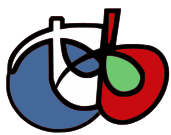
\includegraphics[width=0.6cm]{images/logoIncrust.png}}
\usepackage{fourier}
\usepackage{amsfonts,bm,amsmath,amssymb,ifsym,marvosym,tabularx,array,ifsym}
\usepackage{tikz}
\usetikzlibrary{arrows,fit,backgrounds,positioning,shapes,shadows}
\newcommand{\vns}{Ven$\mu$s}
\newcommand\boxPlot[6] {  \pgfmathsetmacro\rectSize{0.3};  \draw[thick] (#2,#1) -- (#3,#1);  \draw[thick] (#2,#1-\rectSize/2) -- (#2,#1+\rectSize/2);  \draw[thick] (#5,#1) -- (#6,#1);  \draw[thick] (#6,#1-\rectSize/2) -- (#6,#1+\rectSize/2);  \draw[fill=white] (#3,#1-\rectSize) rectangle (#5,#1+\rectSize);  \draw (#4,#1-\rectSize) -- (#4,#1+\rectSize);}
\def\G{\ensuremath{{\cal G}}}
\newcommand{\putat}[3]{\begin{picture}(0,0)(0,0)\put(#1,#2){#3}\end{picture}}
\pgfdeclareimage[height=96mm,width=130mm]{background}{images/fondsClairSansLogo}
\setbeamertemplate{background}{\pgfuseimage{background}}
\subtitle{FOSS4G Europe 2017}
\usetheme{default}
\author{Victor Poughon, Julien Michel, Guillaume Pasero, Rémi Cresson}
\date{2017-07-19}
\title{What's new in Orfeo ToolBox 6.0?}
\hypersetup{
  pdfkeywords={otb},
  pdfsubject={},
  pdfcreator={Emacs 24.4.1 (Org mode 8.2.10)}}
\begin{document}

\maketitle

\begin{frame}
\frametitle{What is Orfeo ToolBox?}
\begin{itemize}
\item \textbf{90+ remote sensing applications}
\item Accessible from C++, Bash, GUI, Python, QGIS, Monteverdi, WPS
\item \textbf{Monteverdi}, a satellite image viewer (hardware accelerated, raw products)
\item A \textbf{C++ library} for image processing, based on ITK
\item \textbf{Big Data} capable, thanks to built-in streaming, multithreading
    and MPI
\item Apache v2.0 license
\item Funded and developed by CNES (French Space Agency)
\item A project of OSGeo since 2017
\item Used at CNES, ESA, mission exploitation platforms,
  remote sensing labs, teaching\ldots
\item Built on the shoulders of giants (ITK, GDAL, OSSIM, OpenCV\ldots)
\end{itemize}

\begin{center}
{\huge\textcolor{red}{\href{http://www.orfeo-toolbox.org}{orfeo-toolbox.org}}}
\end{center}

\end{frame}

\begin{frame}
\frametitle{Incomplete list of OTB functions}

\begin{block}{Pre-processing}
\begin{itemize}
\item Radiometric calibration, orthorectification, resampling (raster and
  vector), pan-sharpening, stereo rectification\ldots
\item Sensor supported: Sentinels, Pléiades, SPOT6, SPOT5, Digital Globe satellites
\item Geometric models (thanks to OSSIM), support for DEM (SRTM or GeoTIFF)
\end{itemize}
\end{block}

\begin{block}{Images and vector manipulation}
\begin{itemize}
\item Formats supported by GDAL (raster and vector), conversion raster/vector
\item Region of interest extraction, of spectral bands, concatenation or splitting\ldots
\item Band math, color mapping, contrast enhancement
\item Linear filtering, Mathematical morphology
\end{itemize}
\end{block}
\end{frame}

\begin{frame}
\frametitle{Incomplete list of OTB functions}

\begin{block}{Feature extraction}
\begin{itemize}
\item Edge detection, scale-invariant feature transform, lines, corners
\item Radiometric indices, textures (Haralick, SFS, PanTex)
\item Local statistics (Flusser moments, Histogram of Oriented Gradient)
\item Keypoints matching (SIFT, SURF\ldots)
\end{itemize}
\end{block}

\begin{block}{Change detection}
\begin{itemize}
\item Classic methods with image metrics comparison
\item Multivariate Alteration Detector
\end{itemize}
\end{block}

\begin{block}{Dimensionality reduction, hyperspectral processing}
\begin{itemize}
\item PCA, NAPCA, ICA, MAF\ldots
\item Dimension estimation, endmembers extraction, Vertex Component Analysis(VCA)
\end{itemize}
\end{block}

\end{frame}

\begin{frame}
\frametitle{Incomplete list of OTB functions}
\begin{block}{Segmentation}
\begin{itemize}
\item Segmentation algorithms: Connected Components, MeanShift,Watershed\ldots
\item Methods to apply those algorithms on large dataset
\item Vector or raster representation which allow Object Based Image Analysis
\end{itemize}
\end{block}

\begin{block}{Classification}
\begin{itemize}
\item 9 supervised methods available (including SVM and Random Forests)
\item Fusion and regularization of classifications
\item K-Means clustering or Kohonen maps
\item Object classification (from a segmentation)
\end{itemize}
\end{block}

\end{frame}

\vspace*{-6.5mm}
\begin{frame}[plain]
\hspace*{-11mm}
    \includegraphics[keepaspectratio,height=1.1\paperheight]{images/mayotte2012.png}
\end{frame}

\vspace*{-6.5mm}
\begin{frame}[plain]
\hspace*{-11mm}
    \includegraphics[keepaspectratio,height=1.1\paperheight]{images/mayotte2013.png}
\end{frame}

\vspace*{-6.5mm}
\begin{frame}[plain]
\hspace*{-11mm}
    \includegraphics[keepaspectratio,height=1.1\paperheight]{images/mayotte_mad.png}
\end{frame}

\vspace*{-6.5mm}
\begin{frame}[plain]
\hspace*{-11mm}
\includegraphics[keepaspectratio,height=1.1\paperheight]{images/saint_paul_lsd.png}
\end{frame}

\vspace*{-6.5mm}
\begin{frame}[plain]
\hspace*{-11mm}
    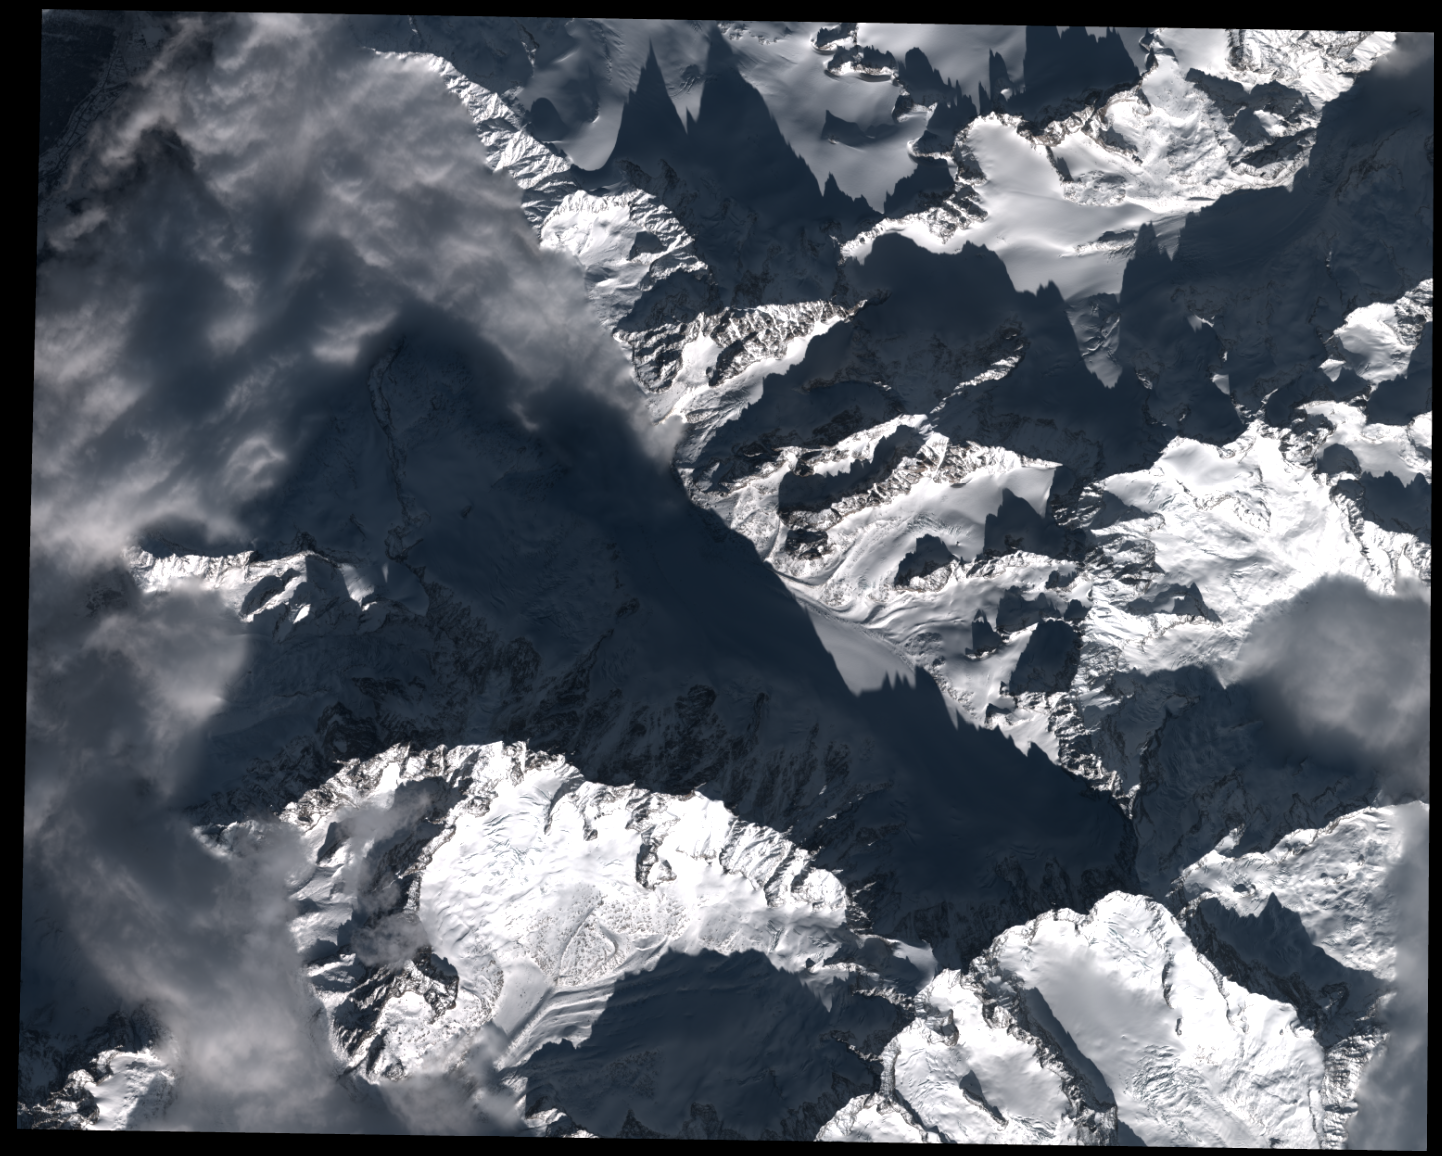
\includegraphics[keepaspectratio,width=1.005\paperwidth,height=1.1\paperheight]{images/argentiere_left.png}
\end{frame}

\vspace*{-6.5mm}
\begin{frame}[plain]
\hspace*{-11mm}
    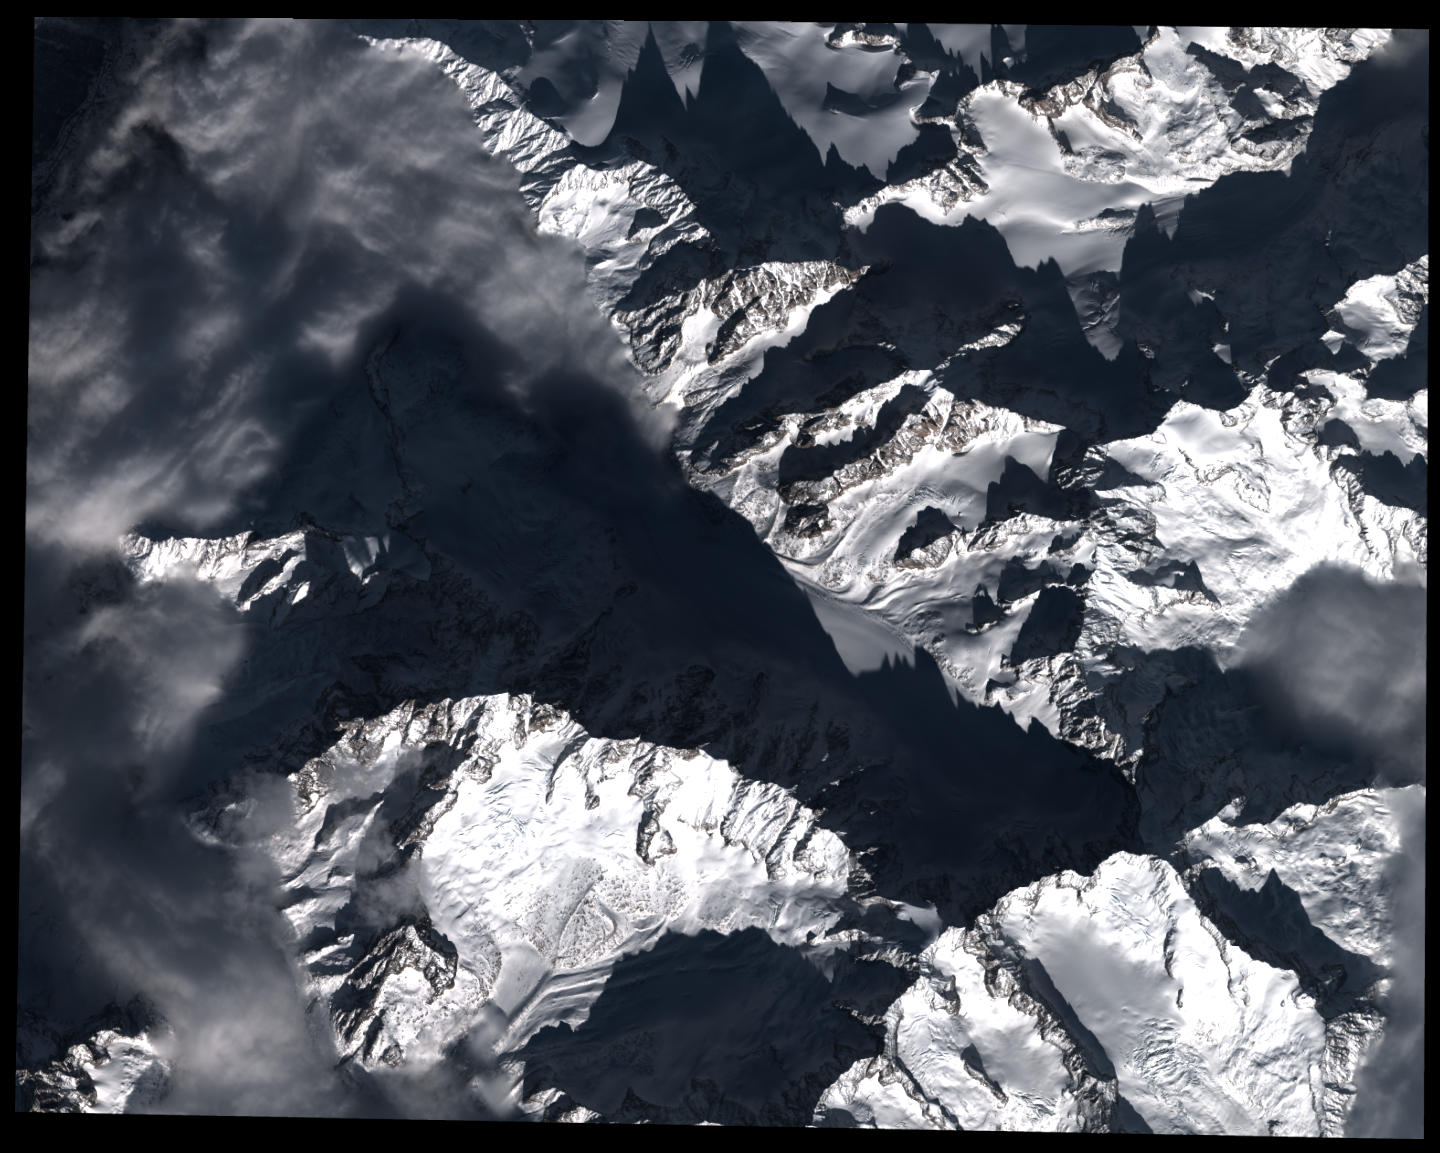
\includegraphics[keepaspectratio,width=1.005\paperwidth,height=1.1\paperheight]{images/argentiere_right.png}
\end{frame}

\vspace*{-6.5mm}
\begin{frame}[plain]
\hspace*{-11mm}
    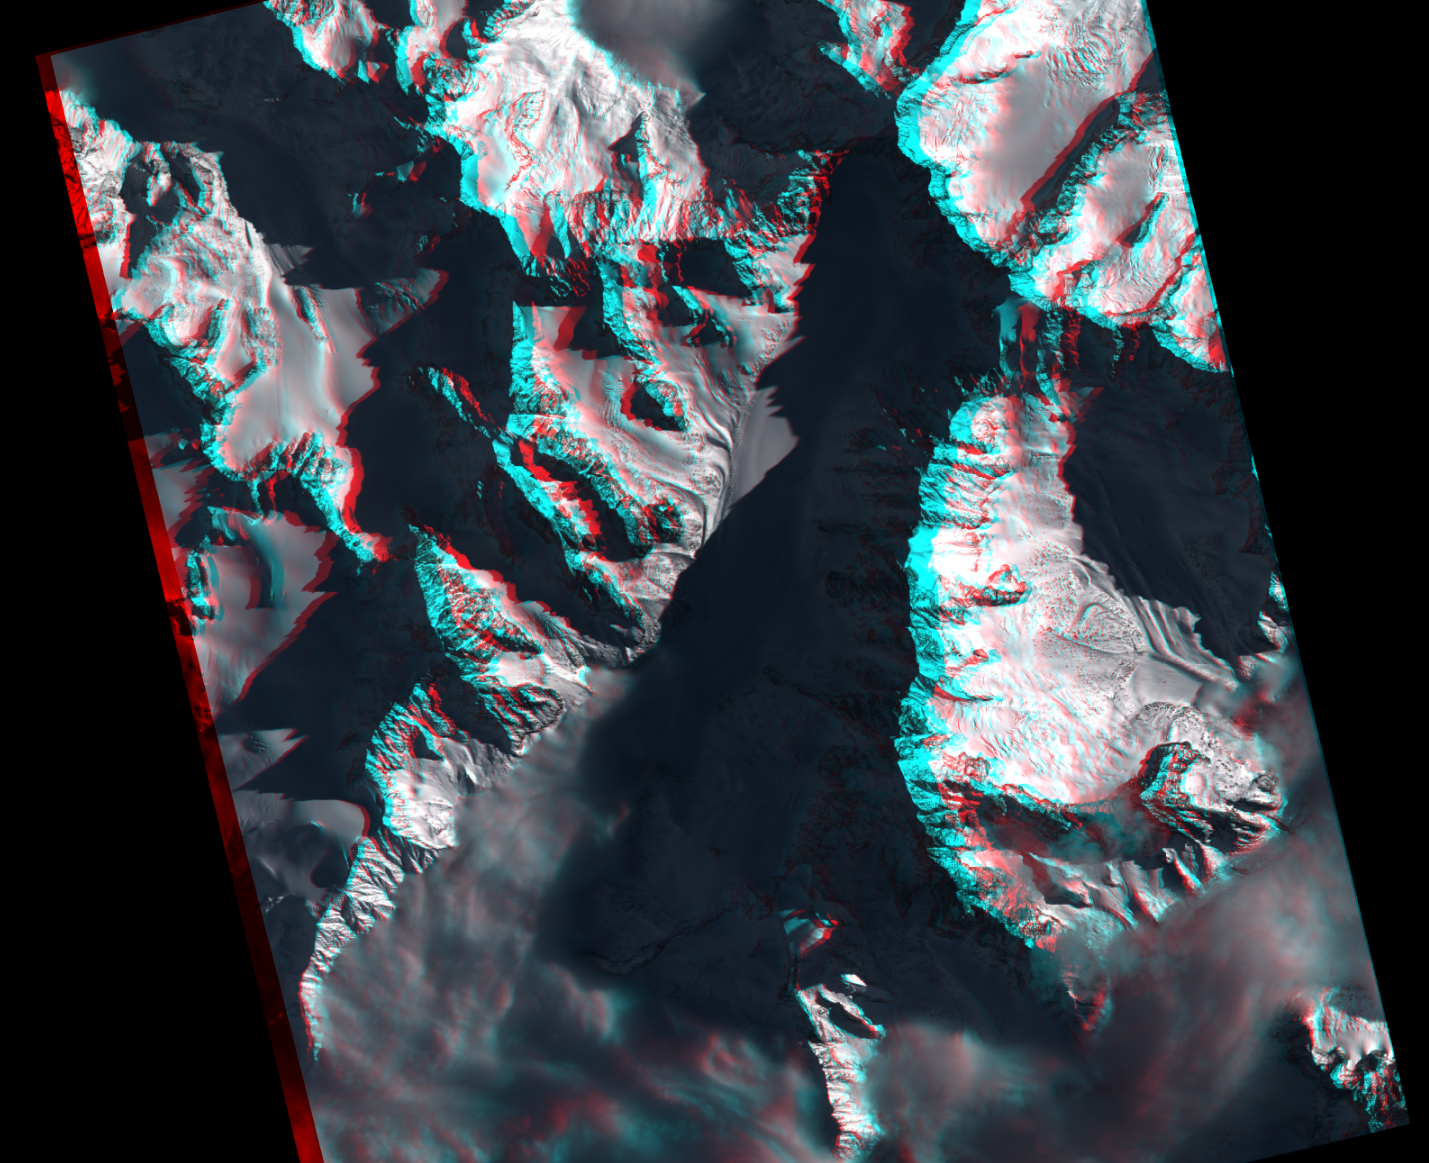
\includegraphics[keepaspectratio,width=1.005\paperwidth,height=1.1\paperheight]{images/argentiere_anaglyphe.png}
\end{frame}


\vspace*{-6.5mm}
\begin{frame}[plain]
\hspace*{-11mm}
    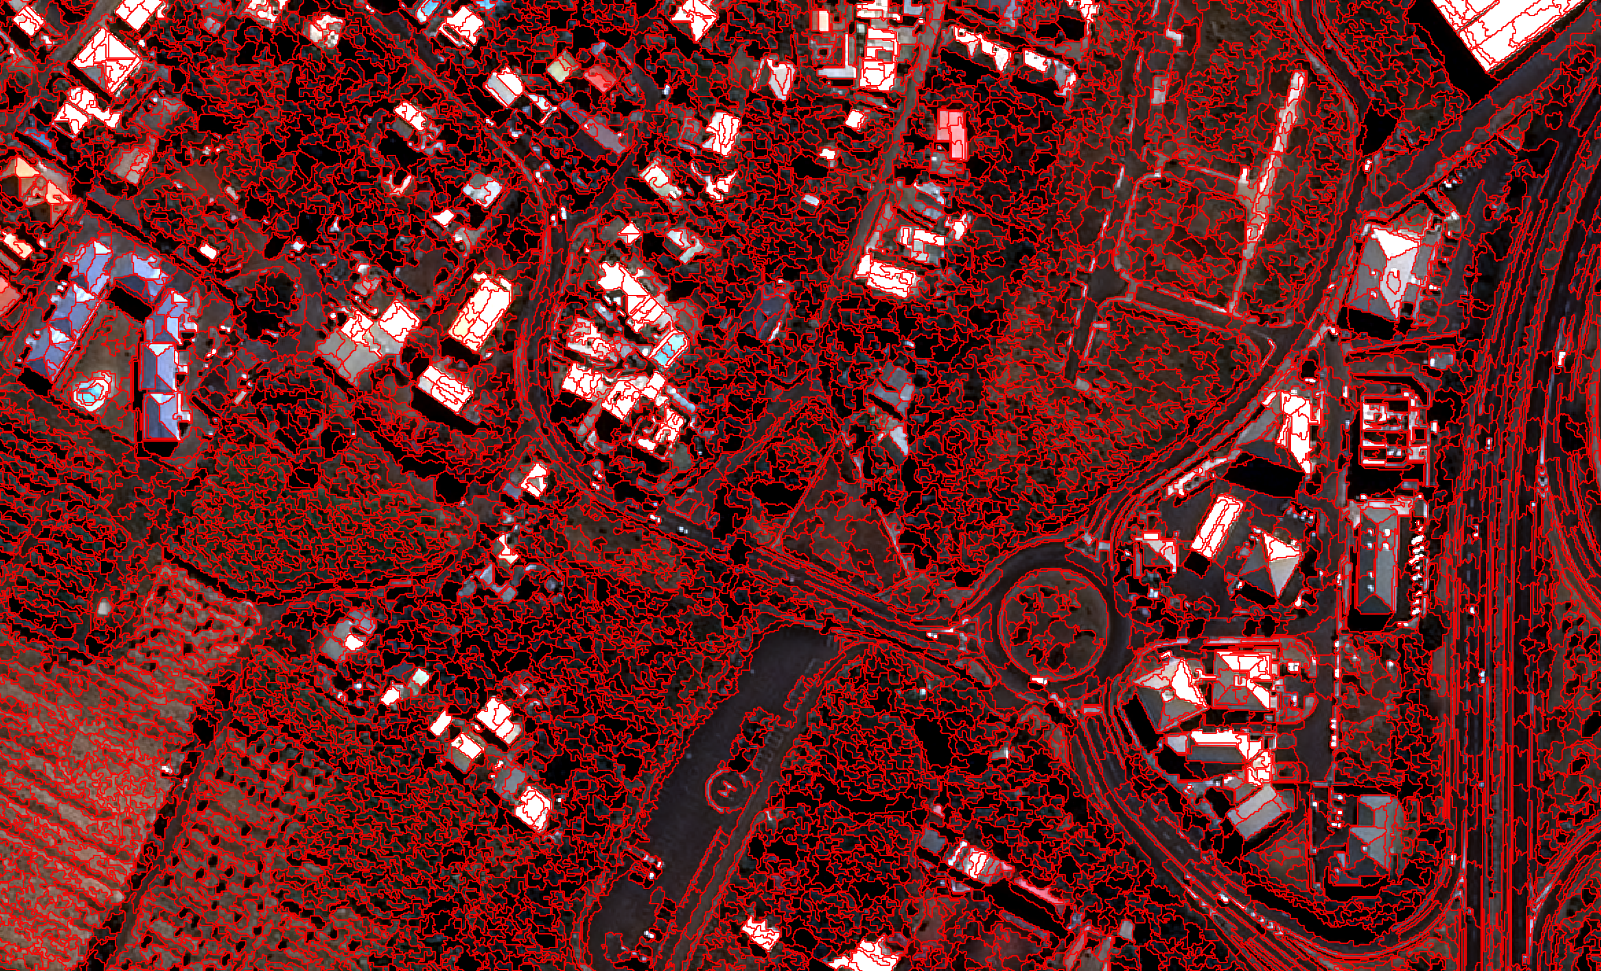
\includegraphics[keepaspectratio,height=1.1\paperheight]{images/segmentation.png}
\end{frame}

\vspace*{-6.5mm}
\begin{frame}[plain]
\hspace*{-11mm}
    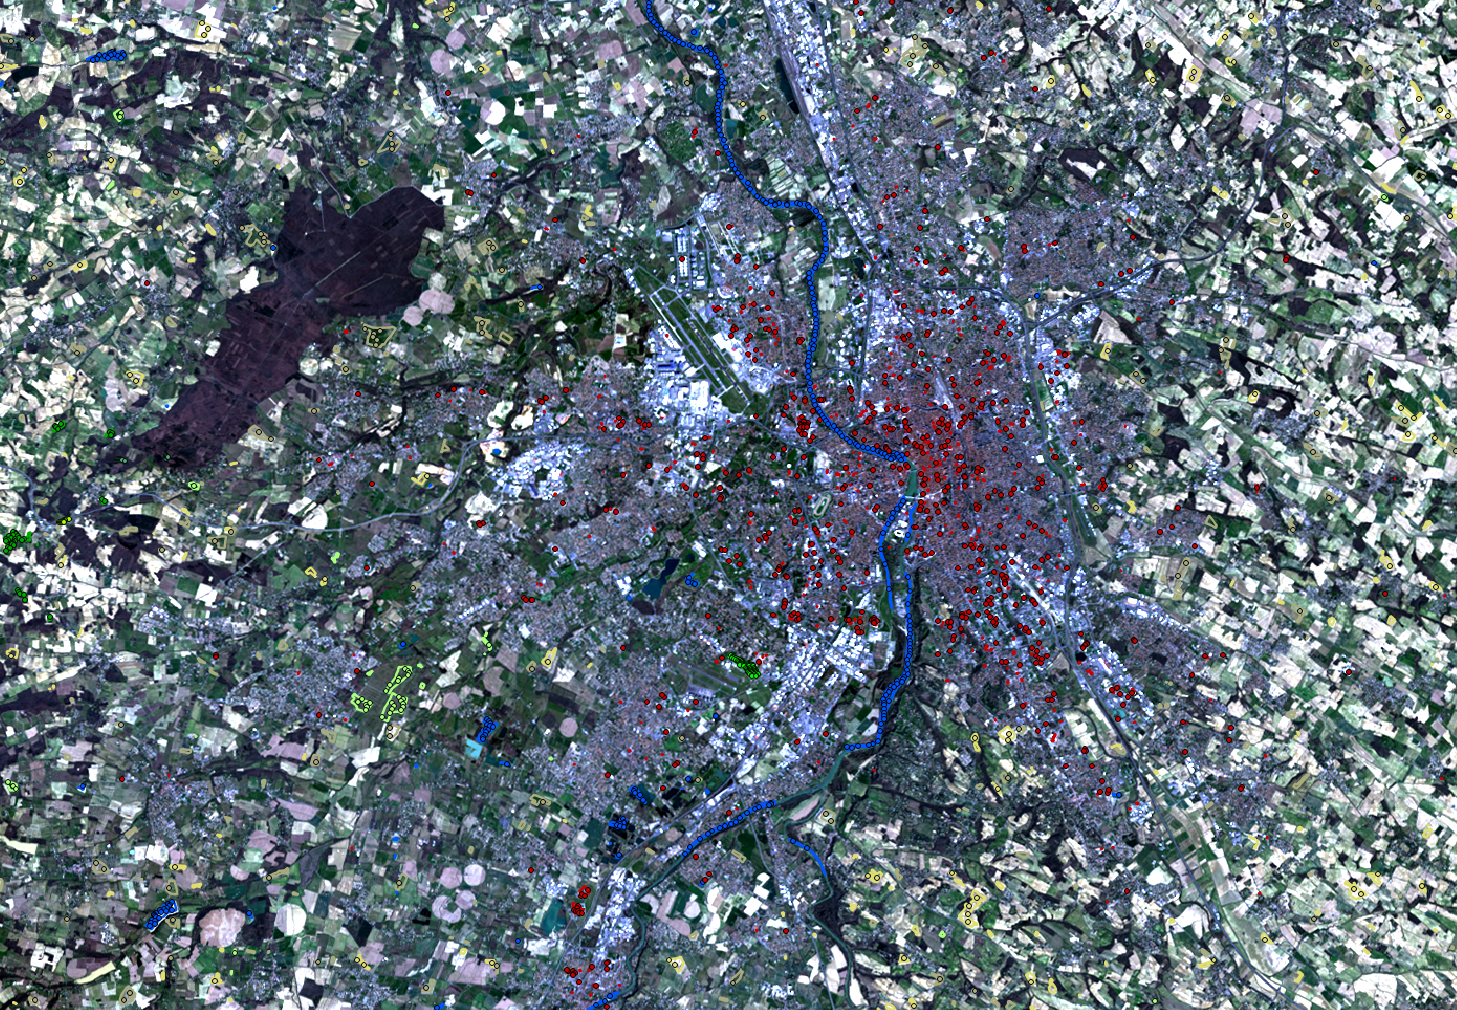
\includegraphics[keepaspectratio,height=1.1\paperheight]{../../Courses/org/WorkshopGuide/Images/samples_selection.png}
\end{frame}


\vspace*{-6.5mm}
\begin{frame}[plain]
\hspace*{-11mm}
    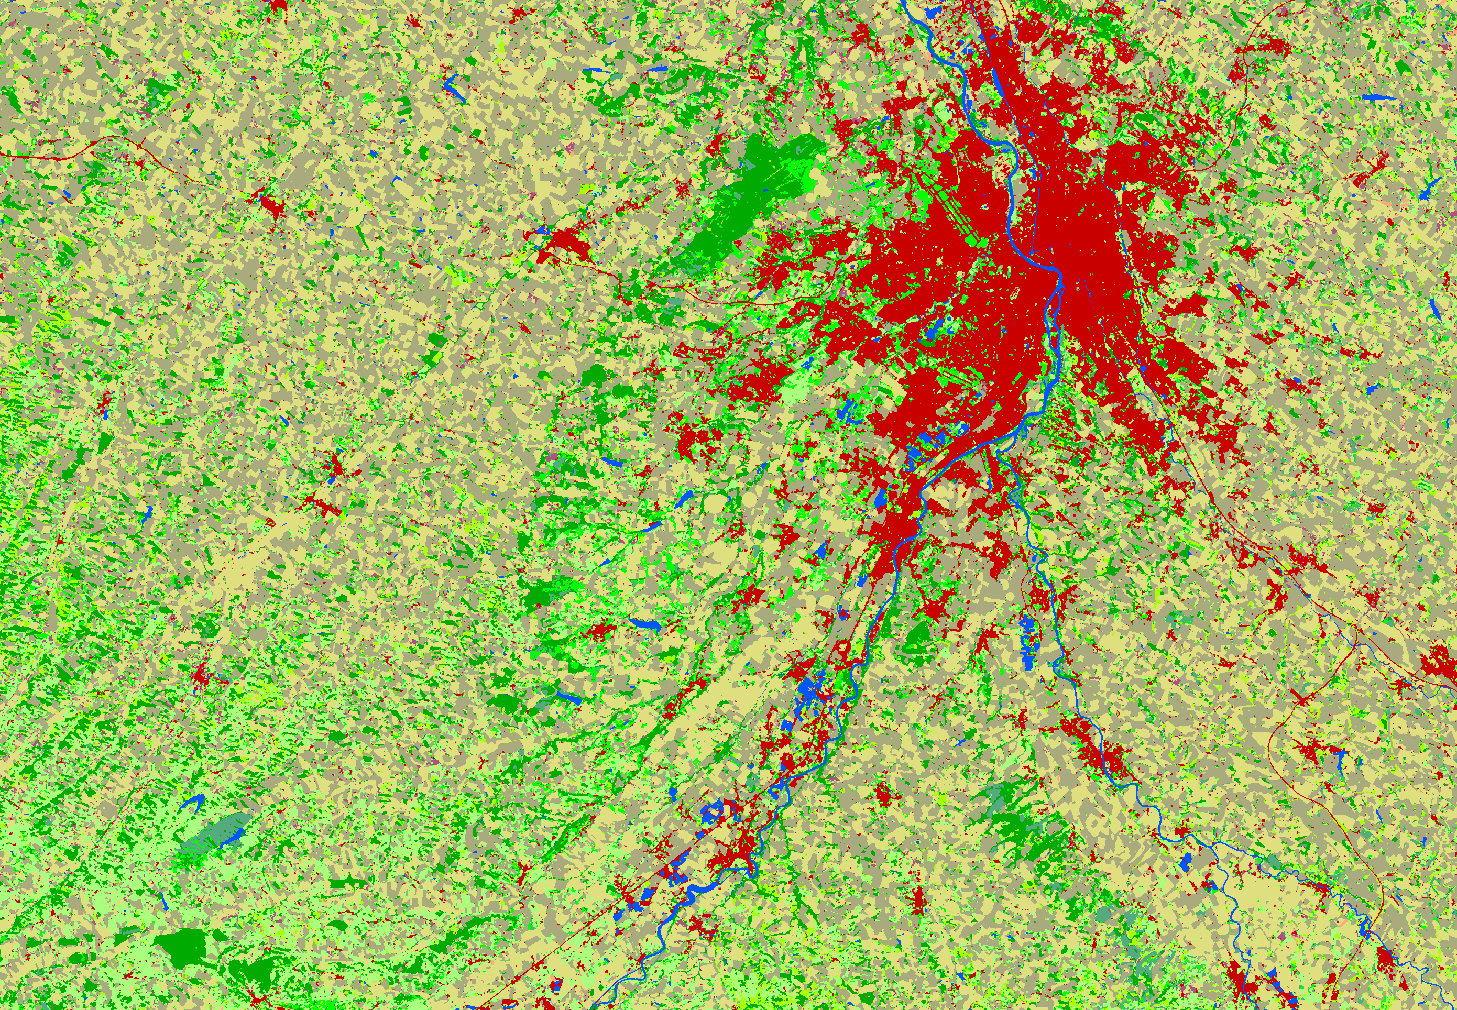
\includegraphics[keepaspectratio,height=1.1\paperheight]{../../Courses/org/WorkshopGuide/Images/final_classification.png}
\end{frame}

\begin{frame}
  \frametitle{Orfeo ToolBox 5.6 \textit{Scincinae}}
  \framesubtitle{Released 2016-07-28}

\begin{itemize}
\item Samples extractor and selection for supervised classification
\item Support for Sentinel-1 products (geometric calibration)
\item Improve Monteverdi OTB-applications display \& search bar
\item MPI pipeline execution
\end{itemize}

\end{frame}

\begin{frame}
\frametitle{Cluster oriented development environment}
\begin{itemize}
\item Remote sensing images processing
\item Abstraction of low-level cluster-related mechanisms
\item Message Passing Interface (MPI) standard
\item Parallel pipelines: read, process, and write using many nodes
\end{itemize}

\begin{center}
\includegraphics[width=0.6\textwidth]{images/mpi1.png}
\end{center}
\end{frame}

\begin{frame}[fragile]
\frametitle{Parallel OTB pipeline with MPI}
  \begin{center}
  \vspace{-0.5cm}
  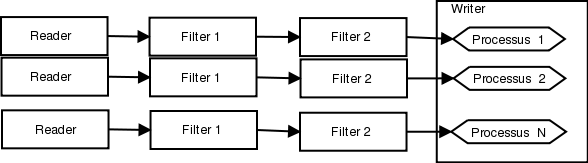
\includegraphics[width=0.6\textwidth]{images/mpi.png}
  \begin{tiny}
\begin{verbatim}
    $ mpirun -np $nb_procs --hostfile $PBS_NODEFILE  \
    otbcli_BundleToPerfectSensor \
    -inp $ROOT/IMG_PHR1A_P_001/IMG_PHR1A_P_201605260427149_ORT_1792732101-001_R1C1.JP2 \
    -inxs $ROOT/IMG_PHR1A_MS_002/IMG_PHR1A_MS_201605260427149_ORT_1792732101-002_R1C1.JP2 \
    -out $ROOT/pxs.tif uint16 -ram 1024

    ------------ JOB INFO 1043196.tu-adm01 -------------

    JOBID           : 1043196.tu-adm01
    USER            : michelj
    GROUP           : ctsiap
    JOB NAME        : OTB_mpi
    SESSION         : 631249
    RES REQSTED     : mem=1575000mb,ncpus=560,place=free,walltime=04:00:00
    RES USED        : cpupercent=1553,cput=00:56:12,mem=4784872kb,ncpus=560,vmem=18558416kb,
    walltime=00:04:35
    BILLING         : 42:46:40 (ncpus x walltime)
    QUEUE           : t72h
    ACCOUNT         : null
    JOB EXIT CODE   : 0

    ------------ END JOB INFO 1043196.tu-adm01 ---------
\end{verbatim}
\end{tiny}
\end{center}
\end{frame}

\begin{frame}
\frametitle{Speedup}

\tiny\begin{itemize}
\item P1 : Orthorectification
\item P2 : Textures Extraction
\item P3 : Pansharpening
\item P4 : RF Image classification
\item P5 : Meanshift filtering
\item P6 : Decompression JP2K
\item P7 : Resampling
\item I/O : Reading / writing
\end{itemize}

\begin{center}
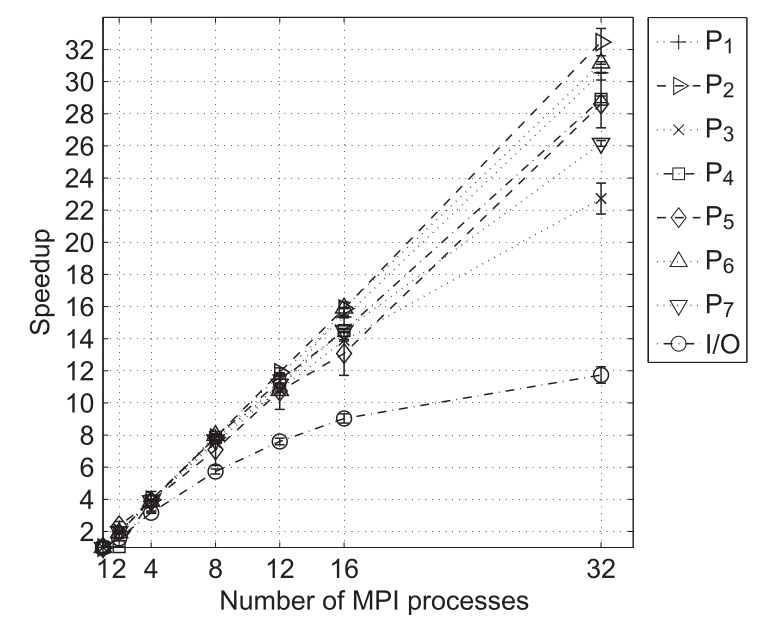
\includegraphics[width=0.6\textwidth]{images/mpi2.png}
\end{center}
\end{frame}

\begin{frame}
\frametitle{I/O bottleneck}
\begin{center}
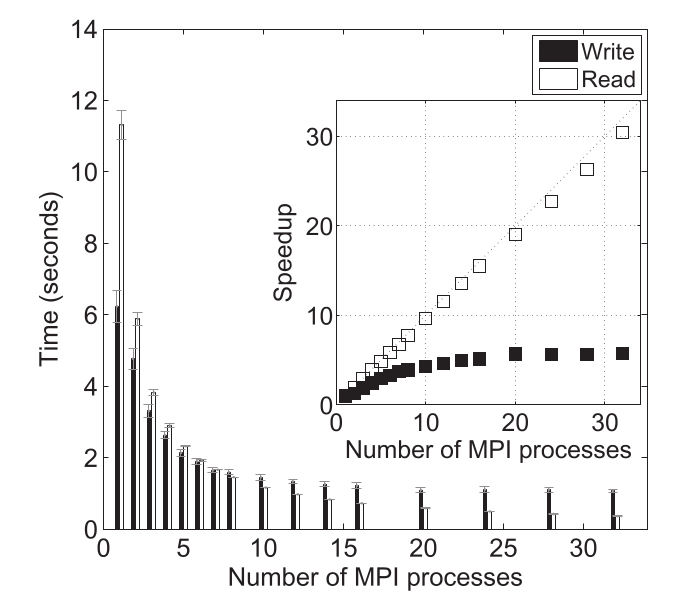
\includegraphics[width=0.6\textwidth]{images/mpi3.png}
\end{center}
\end{frame}

\begin{frame}
\frametitle{Orfeo ToolBox 5.8 \textit{Sphenomorphinae}}
\framesubtitle{Released 2016-11-08}
\begin{block}{OTB}
\begin{itemize}
\item Access to Shark random forests (better performances, parallel learning)
\item Better performances in BandMathX
\item Spot7 support (radiometric and geometric calibration)
\item Applications in-memory connection
\end{itemize}
\end{block}

\begin{block}{Monteverdi}
\begin{itemize}
\item Now part of OTB source code
\item Zoom with mouse wheel without CTRL
\end{itemize}
\end{block}
\end{frame}


\begin{frame}
\frametitle{Orfeo ToolBox 5.10 \textit{Valentine}}
\framesubtitle{Released 2017-02-14}
  \begin{block}{OTB}
    \begin{itemize}
      \item Composite applications framework
      \item TrainImagesClassifier and BundleToPerfectSensor refactoring (composite)
      \item Print corresponding command-line in apps QT GUI
      \item Enhancement of field selector QT component
      \item FFT/DWT application
      \item Texture app now allows for subsampled results (faster)
      \item Packaging remote modules!
    \end{itemize}
  \end{block}

  \begin{block}{Monteverdi}
    \begin{itemize}
      \item Single band color mapping
      \end{itemize}
  \end{block}

\end{frame}

\begin{frame}
\frametitle{Monteverdi on the fly color mapping}
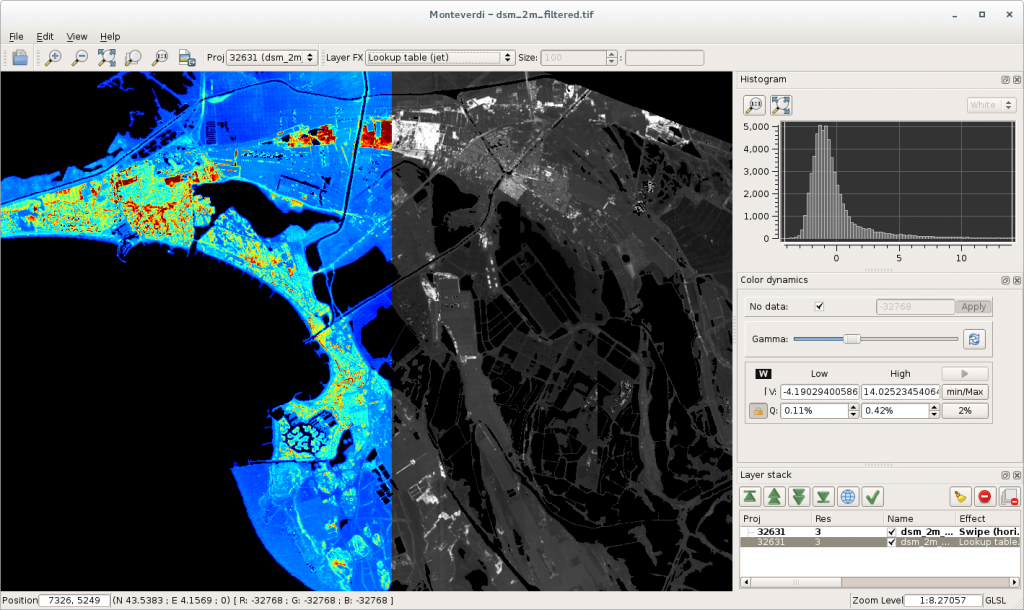
\includegraphics[width=1\textwidth]{images/monteverdi-colormapping.png}
\end{frame}

\begin{frame}
\frametitle{Monteverdi on the fly color mapping}
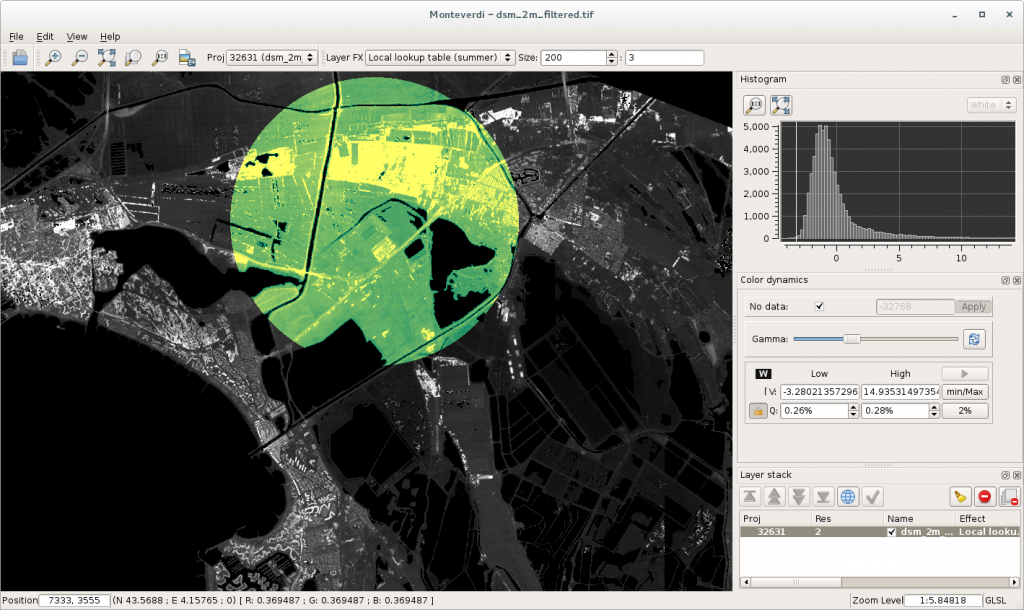
\includegraphics[width=1\textwidth]{images/monteverdi-colormapping2.png}
\end{frame}

\begin{frame}
\frametitle{Automatic command line}
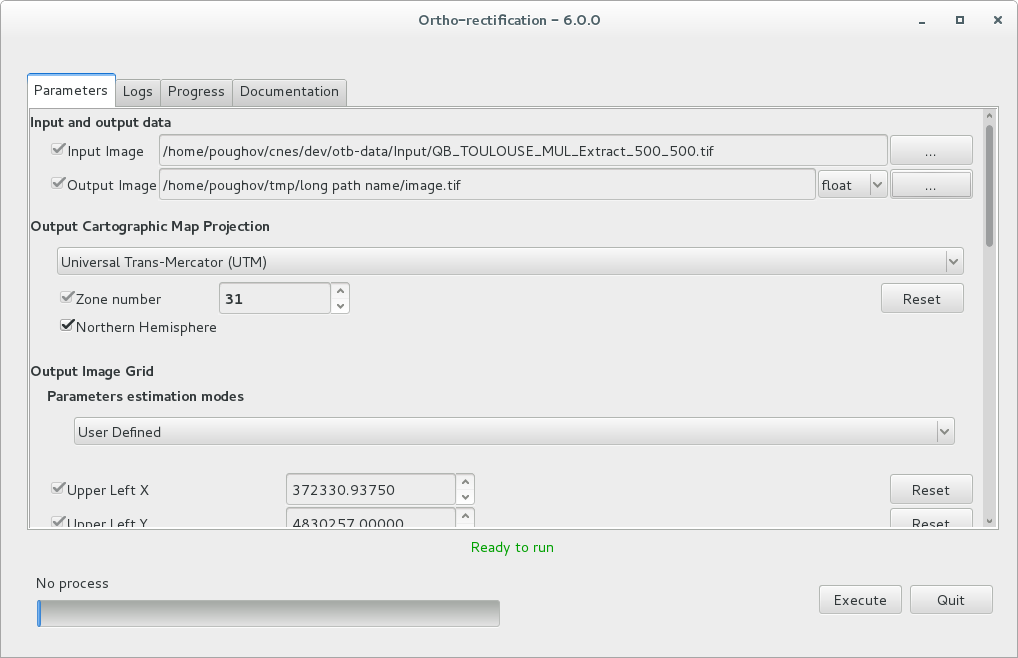
\includegraphics[width=1\textwidth]{images/automatic_command_line1.png}
\end{frame}

\begin{frame}
\frametitle{Automatic command line}
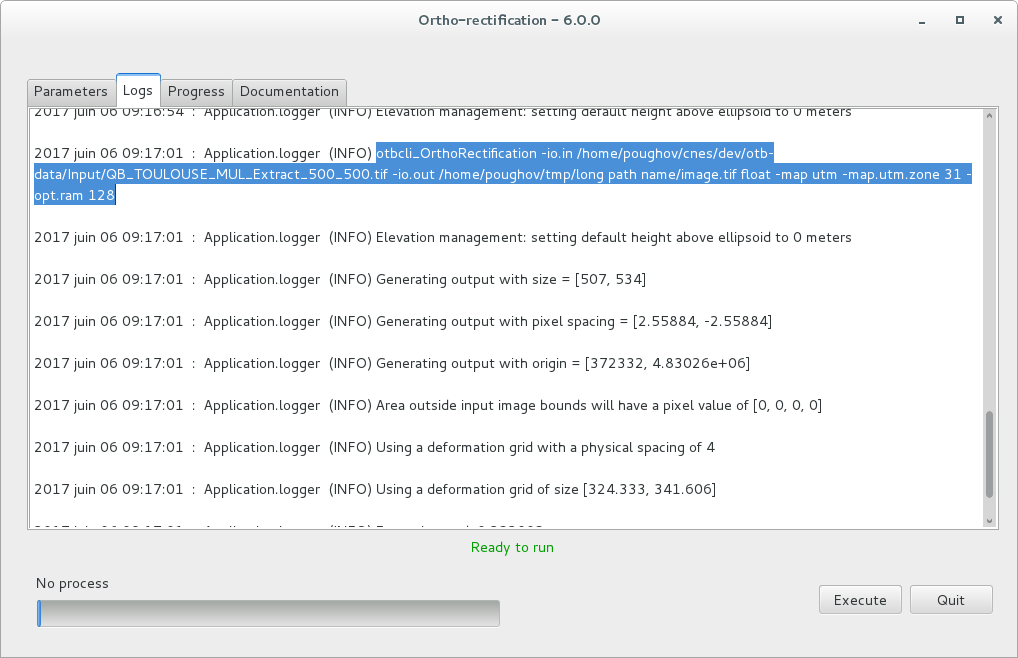
\includegraphics[width=1\textwidth]{images/automatic_command_line2.png}
\end{frame}

\begin{frame}
\frametitle{Orfeo ToolBox 6.0}
\framesubtitle{Released 2017-05-15}
  \begin{block}{OTB}
    \begin{itemize}
      \item Licence change to  Apache v2.0
      \item Sentinel1 IW SLC deburst application
      \item Band selection through extended filenames: \texttt{\&bands=1:4}
      \item Unsupervised classification in framework
      \item Morphological profiles app
      \item Vector files classification app
      \item OpenCV 3.0 support
      \item Deprecated code cleanup (major release)
    \end{itemize}
    \end{block}
\end{frame}

\begin{frame}
\frametitle{Sentinel-1 SLC IW Deburst}
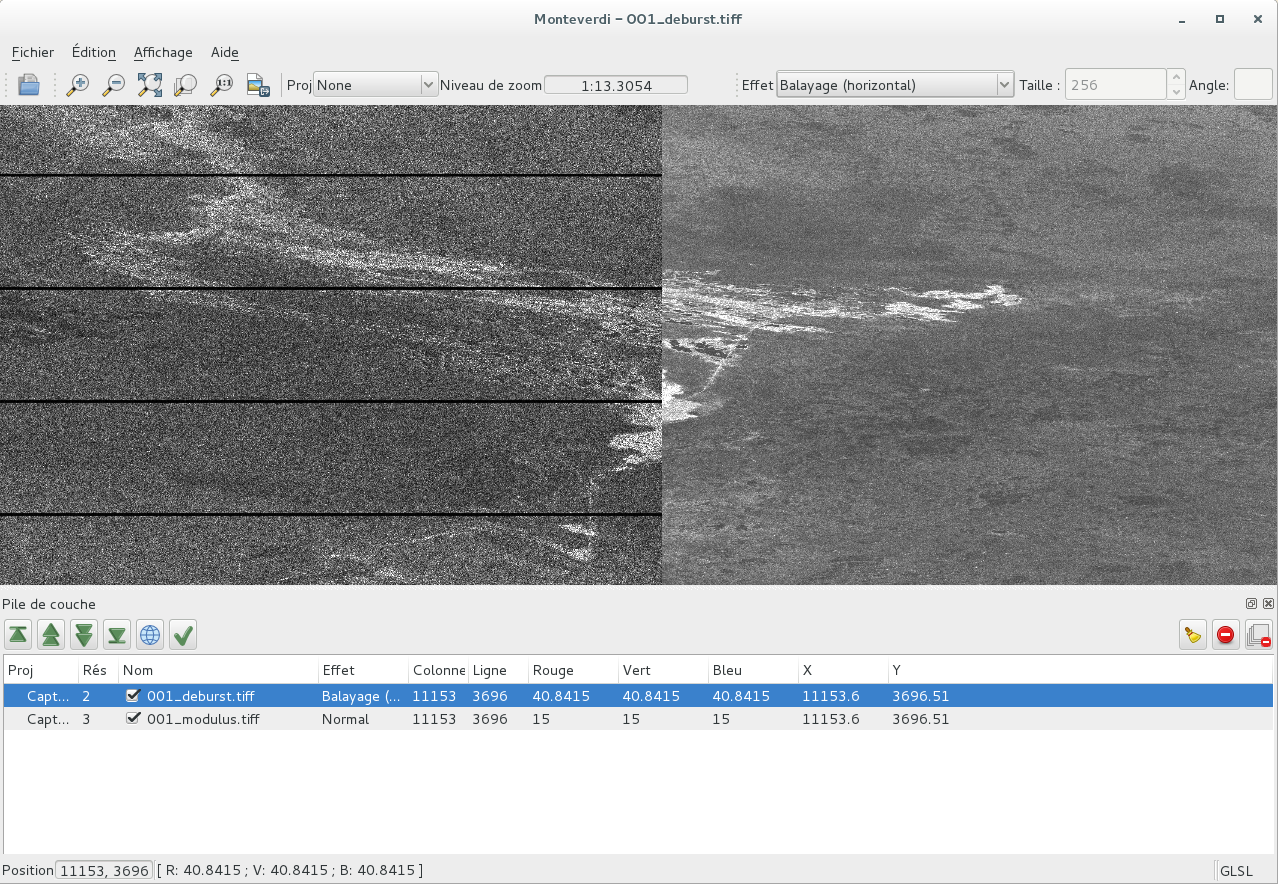
\includegraphics[width=1\textwidth]{images/monteverdi_S1_deburst.png}
\end{frame}

\begin{frame}
\frametitle{Future of Orfeo ToolBox}
\begin{itemize}
\item More features! (Unsupervised learning, OBIA, InSAR, time series image
    stacks)
\item Better QGIS integration
\item Switch to C++14
\item Maintenance (dependencies, binaries packaging, CI)
\item Better documentation
\item We need new Project Steering Commitee members! Are you interested?
\end{itemize}
\end{frame}

\end{document}
